\section{Zadanie 2}
 Rozpoczynaj�c z punktu pracy - przy zerowym zak��ceniu - wyznaczyli�my trzy odpowiedzi skokowe toru zak��cenie-wyj�cie, wykonuj�c skoki sygna�u zak��caj�cego w chwili $k=0$ odpowiednio do warto�ci 10, 20 i 30. Wszystkie odpowiedzi przedstawione s� na rysunku $Rys.\ 2.1$.

%1
\begin{figure}[H]
	\centering
	\begin{tikzpicture}
	\begin{axis}[
	width=5.1in,
	height=1.3in,
	xmin=0,xmax=692,ymin=0,ymax=40,
	xlabel={$k$},
	ylabel={$Z(k)$},
	legend pos=south east,
	y tick label style={/pgf/number format/1000 sep=},
	]
	\addplot[const plot,blue] file {rysunki/data/z10.csv};
	\addplot[const plot,red] file {rysunki/data/z20.csv};
	\addplot[const plot,green] file {rysunki/data/z30.csv};
	\end{axis}
	\end{tikzpicture}
	\begin{tikzpicture}
	\begin{axis}[
	width=5.1in,
	height=1.6in,
	xmin=0,xmax=692,ymin=32,ymax=38,
	xlabel={$k$},
	ylabel={$Y(k)$},
	legend pos=south east,
	y tick label style={/pgf/number format/1000 sep=},
	]
	\addplot[const plot,blue] file {rysunki/data/z0_10.csv};
	\addplot[const plot,red] file {rysunki/data/z0_20.csv};
	\addplot[const plot,green] file {rysunki/data/zad2_z0_30.csv};
	\end{axis}
	\end{tikzpicture}
	\caption{Odpowiedzi skokowe toru zak��cenie-wyj�cie dla r�nych zmian sygna�u zak��caj�cego
	\newline w chwili $k=0$ (w przesz�o�ci zerowe)}
\end{figure}

Wyznaczono charakterystyk� statyczn� ($Rys.\ 2.2.$). W�a�ciwo�ci statyczne obiektu mo�emy okre�li� jako (w przybli�eniu) liniowe.  Wzmocnienie statyczne dla tego toru wynosi w przybli�eniu $\num{0,15}$ - warto�� wsp�czynnika kierunkowego funkcji liniowej b�d�cej charakterystyk� statyczn�.
\begin{figure}[H]
\centering
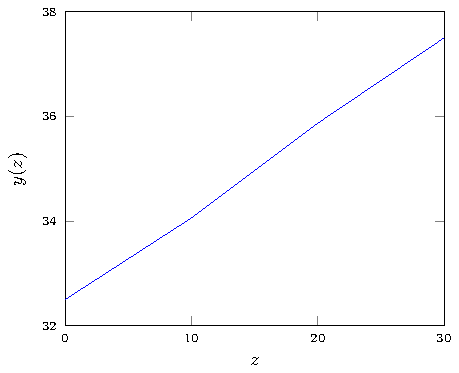
\includegraphics[scale=1]{rysunki/zad2char_st}
\caption{Charakterystyka statyczna - tor zak��cenie-wyj�cie}
\end{figure}